% Load the kaobook class
\documentclass[
	fontsize=10pt, % Base font size
	twoside=true, % Use different layouts for even and odd pages (in particular, if twoside=true, the margin column will be always on the outside)
	open=any, % If twoside=true, uncomment this to force new chapters to start on any page, not only on right (odd) pages
	secnumdepth=1, % How deep to number headings. Defaults to 1 (sections)
]{kaobook}

\usepackage{latt}
% Choose the language
\usepackage[english]{babel} % Load characters and hyphenation
\usepackage[english=american]{csquotes}	% English quotes
\usepackage[utf8]{inputenc}
\usepackage[T1]{fontenc}

% Load packages for testing
\usepackage{blindtext}
%\usepackage{showframe} % Uncomment to show boxes around the text area, margin, header and footer
%\usepackage{showlabels} % Uncomment to output the content of \label commands to the document where they are used

% Load the bibliography package
\usepackage{kaobiblio}
\addbibresource{references.bib} % Bibliography file

% Load mathematical packages for theorems and related environments
\usepackage{kaotheorems}
\usepackage{amsmath,amsthm}

% Load the package for hyperreferences
\usepackage{kaorefs}

\graphicspath{{images/}{./}{assets/}} % Paths where images are looked for


% \usepackage[fencedCode,inlineFootnotes,citations,definitionLists,hashEnumerators,smartEllipses,pipeTables,tableCaptions,hybrid]{markdown}


% \makeindex[columns=3, title=Alphabetical Index, intoc] % Make LaTeX produce the files required to compile the index
% \usepackage[refpage]{nomencl}
\renewcommand{\nomname}{List of Abbreviations}
% \nomrefpage
\makenomenclature


\begin{document}

%----------------------------------------------------------------------------------------
%	BOOK INFORMATION
%----------------------------------------------------------------------------------------

% \titlehead{}
\title[Autoencoders from scratch]{Autoencoders from scratch}
\subtitle{Notes and musings on autoencoders from a PhD student}
\author[Francisco David Charte Luque]{Francisco David Charte Luque\\\texttt{<fdavidcl@ugr.es>}}
% \department{Departamento de Ciencias de la Computación e Inteligencia Artificial}
% \supervisor{Francisco Herrera Triguero\\Francisco Charte Ojeda}
\publicationplace{Granada}
\publicationdate{15 de julio de 2022}
% \date{\underline{Directores de tesis}\\\textbf{Dr. D. Francisco Herrera}\\Soft Computing y Sistemas de Información Inteligentes (Universidad de Granada)\\\textbf{Dr. D. Francisco Charte}\\Sistemas Inteligentes y Minería de Datos (Universidad de Jaén)}
% \publishers{An Awesome Publisher}

%----------------------------------------------------------------------------------------

\frontmatter % Denotes the start of the pre-document content, uses roman numerals

%----------------------------------------------------------------------------------------
%	COPYRIGHT PAGE
%----------------------------------------------------------------------------------------

\makeatletter
\uppertitleback{\@title} % Header

\lowertitleback{
	%\textbf{Disclaimer} \\
	%You can edit this page to suit your needs. For instance, here we have a no copyright statement, a colophon and some other information. This page is based on the corresponding page of Ken Arroyo Ohori's thesis, with minimal changes.
	
	%\medskip
	
	\textbf{Funding} \\
	This doctoral thesis was funded by the predoctoral program Formación del Profesorado Universitario (ref. FPU17/04069) from the Spanish Ministry of Universities.

	\medskip

	\textbf{Copyright} \\
	This book is released under a CC-BY-SA copyright license. This allows you to share and modify it as long as the modifications are released under a similar license.

	To view a copy of the CC-BY-SA code, visit: \\\url{https://creativecommons.org/licenses/by-sa/4.0/}
	
	\medskip
	
	\textbf{Colophon} \\
	This document was typeset with the help of \href{https://sourceforge.net/projects/koma-script/}{\KOMAScript} and \href{https://www.latex-project.org/}{\LaTeX} using the \href{https://github.com/fmarotta/kaobook/}{kaobook} class.
	
	\medskip
	
	% \textbf{Publisher} \\
	% First printed in May 2019 by \@publishers
}
\makeatother

%----------------------------------------------------------------------------------------
%	DEDICATION
%----------------------------------------------------------------------------------------

\dedication{\itshape
% This is only a foretaste of what is to come, and only the shadow of what is going to be.
	Machines take me by surprise with great frequency. \\
	\flushright -- Alan Turing
}

%----------------------------------------------------------------------------------------
%	OUTPUT TITLE PAGE AND PREVIOUS
%----------------------------------------------------------------------------------------

% Note that \maketitle outputs the pages before here
\makeouterpage
\maketitle

\pagestyle{pagenum.scrheadings}

%----------------------------------------------------------------------------------------
%	PREFACE
%----------------------------------------------------------------------------------------

\chapter*{Abstract}

\blindtext

\chapter*{Resumen}

\blindtext

%----------------------------------------------------------------------------------------
%	TABLE OF CONTENTS & LIST OF FIGURES/TABLES
%----------------------------------------------------------------------------------------

\begingroup % Local scope for the following commands

% Define the style for the TOC, LOF, and LOT
%\setstretch{1} % Uncomment to modify line spacing in the ToC
%\hypersetup{linkcolor=blue} % Uncomment to set the colour of links in the ToC
\setlength{\textheight}{230\vscale} % Manually adjust the height of the ToC pages

% Turn on compatibility mode for the etoc package
\etocstandarddisplaystyle % "toc display" as if etoc was not loaded
\etocstandardlines % "toc lines as if etoc was not loaded

\tableofcontents % Output the table of contents

\listoffigures % Output the list of figures

% Comment both of the following lines to have the LOF and the LOT on different pages
\let\cleardoublepage\bigskip
\let\clearpage\bigskip

\listoftables % Output the list of tables

\endgroup

%----------------------------------------------------------------------------------------
%	MAIN BODY
%----------------------------------------------------------------------------------------

\mainmatter % Denotes the start of the main document content, resets page numbering and uses arabic numbers
\setchapterstyle{kao} % Choose the default chapter heading style

\setchapterpreamble[u]{\margintoc}
\chapter{Introduction}
\labch{intro}


Current trends in collection of data are increasing, with more and more human activities producing machine-readable information, such as product reviews \sidecite[1.8cm]{fang2015sentiment}, posts on social media \sidecite[2.7cm]{balaji2021machine}, medical images \sidecite[3.45cm]{willemink2020preparing}, industrial machinery sensor data \sidecite[4.72cm]{gao2015survey}, and more. Automatic processing of data makes it easier to obtain  results fast and saves hours of human labor which can be freed for other purposes or dedicated to tasks which cannot be automated. The speed provided by current computation resources also opens new possibilities for leveraging the available data, achieving extraction and manipulation of information at levels infeasible by human hand.

The study of problems, tools and solutions related to data integration, processing and analysis has been recently known as data science \sidecite[1.5cm]{dhar2013data}, a field which overlaps branches of mathematics, statistics and computer science, among other disciplines. Current data science applications are present everywhere, from the most industrial settings to direct final user access, and range from machinery fault detection \sidecite{carvalho2019systematic}, to medical diagnosis assistance \sidecite{erickson2017machine}, customer loyalty in retail \sidecite{ma2020machine} and photograph enhancing \sidecite{wang2020deep}.

The general objective in a data science problem is to model a real world scenario based on the collected data and use the resulting model to provide some information to the end user, for example, a category or label, a ranking, an association or a transformed version of the original data. This is a process that encompasses all steps from data acquisition, to its preparation, processing and analysis. In this context, a wide variety of computer algorithms are used to manipulate and process data. The study and development of these techniques that allow machines to distill knowledge from data are known as \textit{machine learning}.

\section{Problem setting}

There are several stages that compose the process of solving a data science problem, represented visually in Figure~\ref{fig:kdd}. A great part of the time spent, usually the longest, consists in preparing and preprocessing the available data in order for the posterior learning techniques to extract the maximum possible amount of information and ensure the new knowledge is valid \sidecite{domingos2012few}. There exist several traits of the data that can be manipulated to facilitate the work of learning algorithms: missing values, noisy instances, class imbalance, among others \sidecite{garcia2015data}.

\begin{figure}
    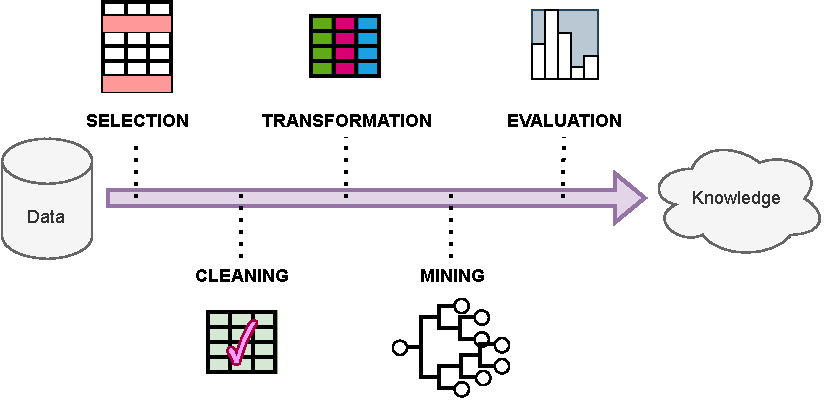
\includegraphics[width=\linewidth]{images/kddprocess.pdf}
    \caption{\label{fig:kdd}Process of knowledge discovery in databases (KDD)}
\end{figure}

The set of features, that is, the specific representation of each instance in a dataset, is one aspect which machine learning models can be specially sensitive to.

Features that may characterize an event or object adequately for humans may not be ideal for machines to process. For example, a string of text may have meaning for a reader but for the machine it is just a sequence of characters whose semantics are not easily processed in that format. Similarly, an image can be expressed as a series of color values which, if shown on a screen, will display something intelligible for a person's eye, but those values do not hold direct relation to what is contained in the image itself.

\begin{marginfigure}
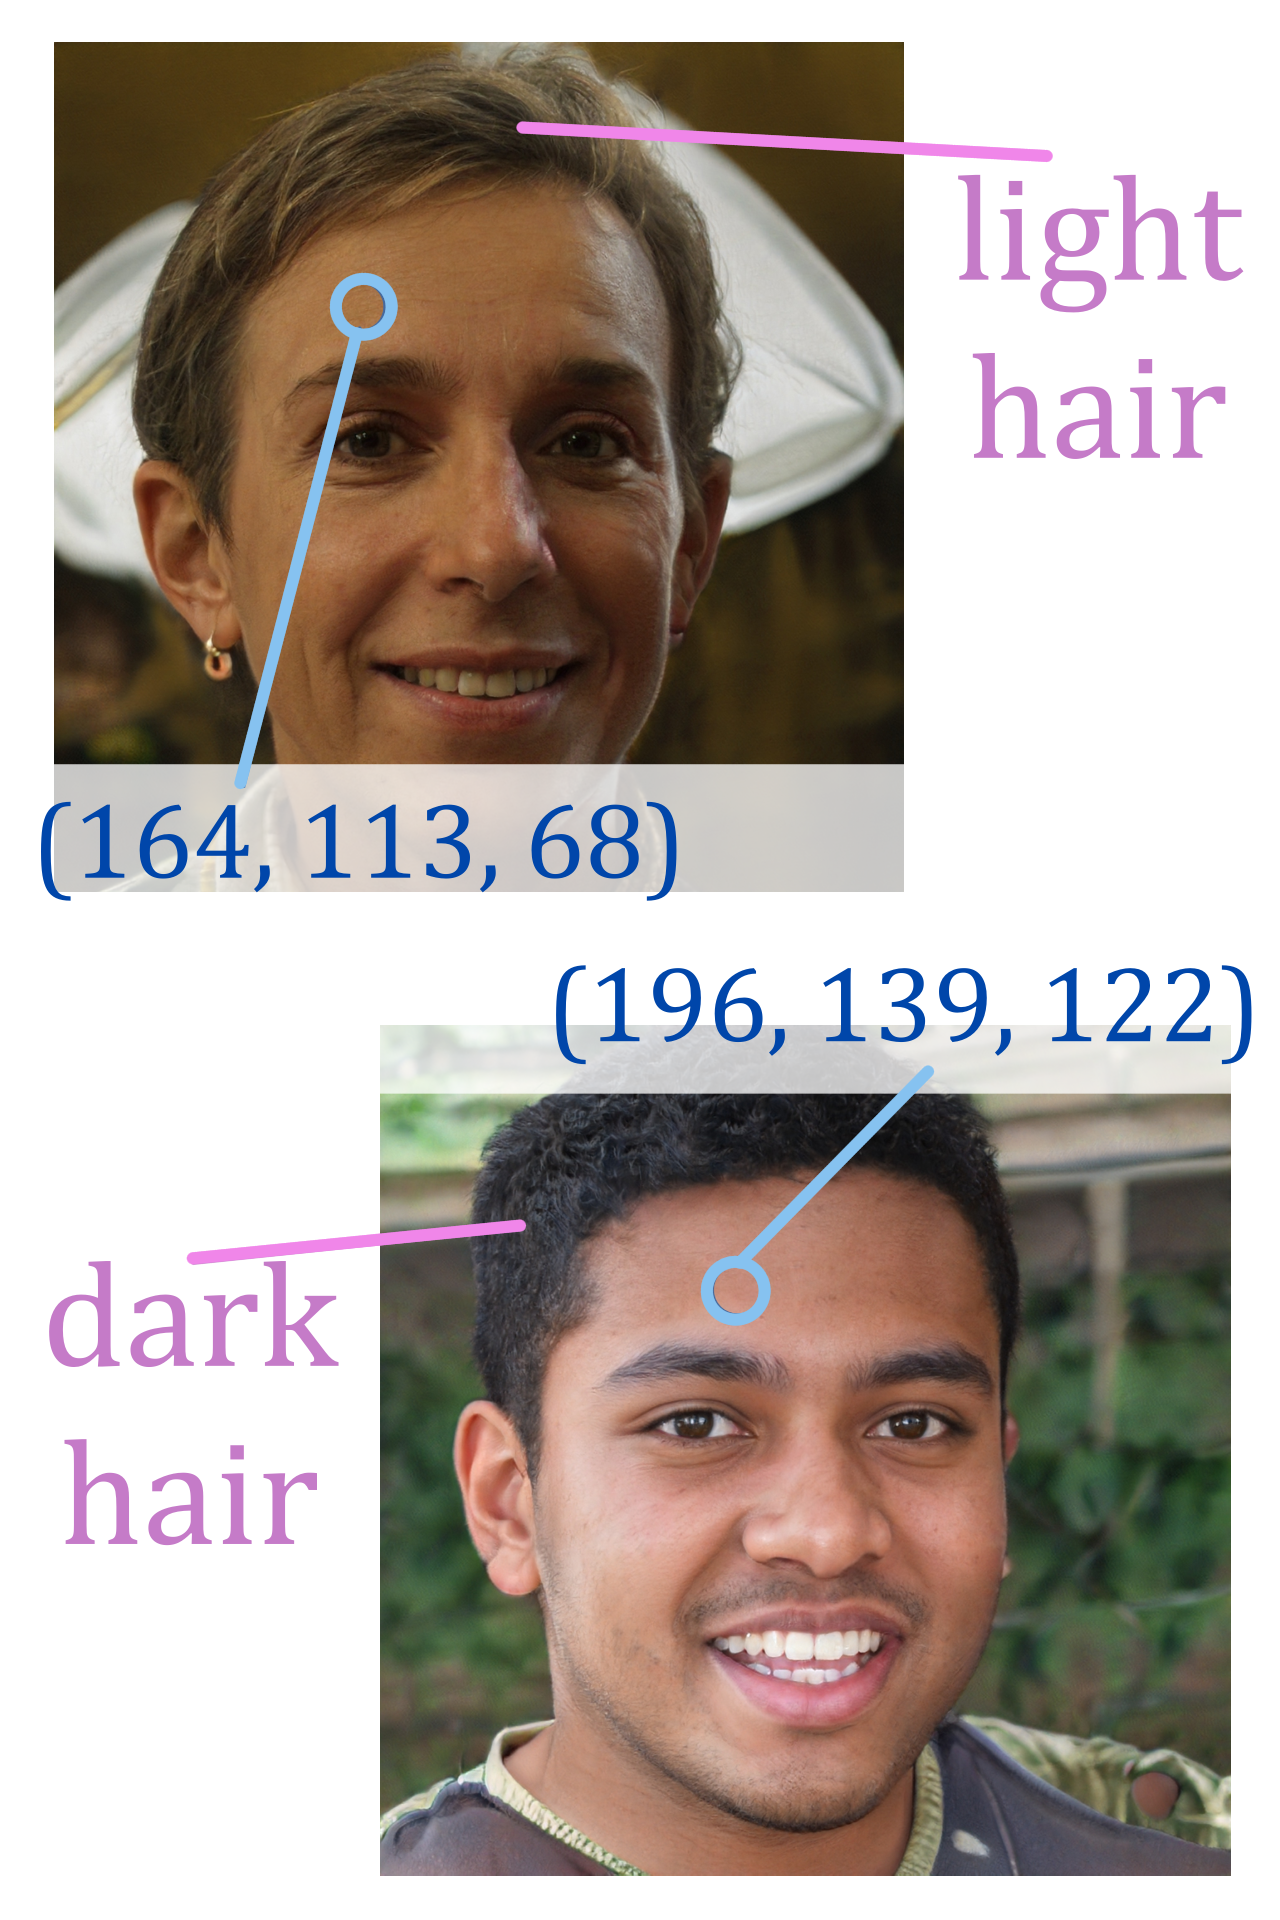
\includegraphics[width=\linewidth]{latentvariables.png}
\caption{\label{fig:latentfaces}Two randomly generated images from \url{https://thispersondoesnotexist.com}. In blue, available features such as the color values of some pixels. In pink, latent variable values (such as \textit{hair tone}) that are not directly represented in the data but influence those color values.}
\end{marginfigure}

Furthermore, the techniques used for collecting data can only produce the observable variables in a dataset, but there may be interesting, hidden variables which influence the data in a clearer way. This is a concept known in statistics as \textit{latent variables} \sidecite{borsboom2008latent}. For example, the value  ``blond'' for the latent variable ``hair color'' might determine the color value of many pixels in an image of a person's face, but those are also influenced by overall lighting and contrast, so the hair color of a person cannot be deduced by just extracting a couple of pixels (see Figure~\ref{fig:latentfaces} for an example). It would be desirable to obtain the meaningful features, but a learning mechanism that takes all observable features into account is needed for these to be extracted.

Providing a learning algorithm with unprocessed features usually leads to sub-par performance due to several potential issues: different scales, presence of noisy variables, redundant information, useful information that is obscured and not directly represented, as well as irrelevant information. All of this may confuse a learning method which initially might consider all variables equally relevant.

Other possible obstacles that one may come across when inspecting the features of a dataset are difficult classes, also known as data complexity \sidecite{cano2013analysis}. This scenario arises when the variables do not provide sufficient information to allow class separation, the relations between variables and the target are highly nonlinear, or other circumstances prevent a learning method from inferring an adequate mapping from the input features to the target variable.

As a consequence, much time can be spent manually engineering features according to what the practitioner believes the learning method will adapt best. However, this is a process that requires experience and usually involves many attempts at improving results. Instead of this, a new task can be performed by machine learning techniques before the actual knowledge extraction, called \textit{feature learning} or more broadly \textit{representation learning} \sidecite{bengio2013representation}. 

Feature learning alleviates a notable amount of manual labor and dataset manipulation although, of course, implies that the user know about feature learning methods and their operation. There exists a very diverse array of methods, ranging from simple principal component analysis (PCA) to more complex manifold learning methods.

However, not every feature learning method can solve every task. Most of them have a specific criterion that they optimize, such as maximum variance in the case of PCA, point reconstruction from its neighbors as in locally linear embedding \sidecite{LLE}, or shortest-path distances between points as in Isomap \sidecite{Isomap}. The objective function of each method determines which behavior will be found in the extracted representation, with little to no room to customize it. There may be situations where it is necessary for the learned variables to adjust to certain properties and, ideally, the feature extraction method should allow to enforce those properties.

\section{Tools}

The main set of tools that are used to tackle problems along this work is \textit{deep learning}, a subset of machine learning focused on algorithms which extract successive transformations of the data until a solution to the task is reached.

Deep learning originates from the concept of artificial neuron, which takes some inspiration on the biological nervous system \sidecite{mcculloch1943logical}. The perceptron, a probabilistic model of the brain, was developed drawing from this abstract neuron \sidecite{rosenblatt1958perceptron} and current artificial neural networks are simply generalizations of the multi-layer perceptron (MLP). For a long time, neural networks were very inefficient to train compared to other machine learning methods, and they were not used for many applications as a result.

The resurgence of neural network models for machine learning has happened more recently due to the fact that their optimization had much higher computational cost than other, classical machine learning models. Thus, more efficient optimization strategies in combination with much more powerful hardware (leveraging the computing capacities of modern GPUs) have allowed to train complex deep models which were unfeasible before.

Nowadays, deep learning is used to extract the contents of images, natural language and speech (as well as produce them) in a wide range of applications, from small fitness devices to autonomous vehicles. It is also very present in research fields ranging from medicine to computer security. It powers translation systems \sidecite{deepl}, search engines \sidecite{SHU19991} and virtual assistants \sidecite{mycroft}. 

The main advantage of deep learning against traditional machine learning methods is being able to automatically transform raw data into useful representations that depict more complex, high-level concepts. This stage is usually performed manually when approaching machine learning problems with other models.

Since deep learning models perform their own representation learning while training to solve other tasks, one possible use for these models is the extraction of said representations. One can either extract these \textit{deep features} from neural networks which are trained for a different purpose or build a deep learning model dedicated to just learning a new, more useful representation. The latter approach will be our focus during most of this thesis, using a specific category of models known as \textit{autoencoders}.

\section{Motivation}

The questions that we are trying to tackle throughout this thesis can be summarized as follows:

\begin{itemize}
    \item How can representation learning be approached with deep neural models?
    \item What benefits can be obtained by transforming data into an appropriate representation?
    \item Can specific behavior be induced within the transformations, such as separating different classes?
\end{itemize}


% - the potential of deep neural models over other methods for feature learning

As the trends in usage of deep learning models to solve machine learning problems continue to increase, we focus our interest in their potential to not only tackle supervised problems such as classification, regression or detection, but also wider problems where solutions are not so easily validated, such as feature learning. Since deep learning allows the integration of the feature extraction stage directly within the predictor itself, these types of models should be valuable feature learners for other tasks as well.

% - interest in how to adapt feature generation for different purposes, e.g. multiple outputs

Deep neural models dedicated to generating new feature sets could be adapted, as a result, to different purposes. For instance, one could search for feature spaces where ``ordinary'' data points are very cohesive, and thus anomalous inputs would be easy to identify. Similarly, a transformation of features could allow for better separation of different classes, better distinction between noise and signal, or more meaningful traits that relate to all the original variables.

% - interest in multi-view problems

Another potential use of feature learning models that catches our interest is the possibility of capturing more than one aspect of each problem instance, which translates to different \textit{views} of the problem, for example, image and text. These views could be processed by different learners or special algorithms, but one could build feature learners that combine the available information into a more machine-ready feature vector.

% - interest in interpretable models

A current conflict of deep learning models with several areas of interest in machine learning, such as medical applications, is the fact that most are essentially black boxes \sidecite{fong2017interpretable}. This means that the behavior of a trained model is obscured by the intrinsic structure and is thus unintuitive for humans to comprehend. As a result, there is much interest in explaining and justifying the behavior of these models. Enabling the use of interpretable classifiers and regressors such as decision trees by means of better dataset representations can be one way of avoiding black boxes in these contexts.

\section{Objectives}

All the research developed along this work has been revolving around the general aim of improving how autoencoders can achieve a better representation of data in order to extract more reliable models from it. 

As a result, the specific objectives that we posed throughout the course of the thesis were the following:

\begin{itemize}
    \item To acquire a deep understanding on how autoencoders work, how they differ from other feature extraction techniques, and the different approaches to learn new features with them.
    \item To facilitate the use of autoencoders by unspecialized users, improving on previous implementations in efficiency and ease of use.
    \item To explore different types of supervised learning problems further from the classical binary (positive/negative) prediction schemes or regression tasks.
    \item In the context of supervised problems, to develop new ways of optimizing autoencoders so that generated features are able to separate different classes better.
\end{itemize}

Additionally, there are several tangential issues that were studied due to the interesting relation to the main topic and the opportunity to work on real world problems. These are as follows:

\begin{itemize}
    \item To identify areas of application where autoencoders are able to provide solutions without the need of additional modelling.
    \item To evaluate and compare different encoder-decoder architectures for different purposes .
    \item To analyze whether ensembling several encoder-decoder methods can provide better solutions.
\end{itemize}

\section{Thesis structure}

This work comprises several original introductory chapters presenting the necessary theoretical concepts and the basics on how these are put to practice, as well as reproductions of five articles published in peer-reviewed journals, each of them related one or more of the previously established goals for this thesis.

The rest of this document is organized as follows: %contains all the needed information to develop the posed questions and provide enough context in order to understand the work that has been realized throughout the thesis.

\begin{itemize}
    \item Chapter~\ref{ch:theory} describes the basic theory that lies under the subsequent works and the specific models that are developed and used.
    \item Chapter~\ref{ch:practical} explains the practicalities of implementing and training deep learning models, especially autoencoders.
    \item Chapter~\ref{ch:summary} outlines the main results obtained during the research period, providing context and connections among the articles that are reproduced next.
    \item Article~\ref{ch:paper1}, the first of the journal articles, is a guide on the inner workings of autoencoders, their variants, how to design and how to implement them.
    \item Article~\ref{ch:paper2} describes into detail the software developed with the objective to facilitate the use of autoencoders.
    \item Article~\ref{ch:paper3} is a review of the current state of the art in supervised learning further from the standard problems.
    \item Article~\ref{ch:paper5} covers the most popular applications of autoencoders apart from classification, with concrete examples and guidelines.
    \item Article~\ref{ch:paper6} improves the applicability of autoencoders in classification problems by developing new loss functions which help reduce data complexity.
    \item Lastly, Chapter~\ref{ch:conclusions} draws some conclusions and closing statements on the developed work.
\end{itemize}
\setchapterpreamble[u]{\margintoc}
\chapter{Theoretical foundation}
\labch{theory}

Machine learning covers a set of problems and tools that overlaps several disciplines. As such, in order to tackle machine learning problems, it is necessary to lay some foundations which help grasp all the concepts involved. Even though this is a rapidly evolving field, there are fundamental topics that remain applicable.

The objective of this chapter is to provide the reader with the definitions, descriptions and examples that allow to understand the rest of this work. We will try to assume little-to-no prior knowledge about machine learning, thus making it as accessible as possible. The following sections go over the basic subjects of machine learning, build the core concepts of deep learning and arrive to the main tools that will be used along the rest of this book, autoencoders.

\section{Machine learning fundamentals}[ML fundamentals]

Machine learning\index{machine learning} differs from other kinds of computer science disciplines in that its objective is not to give precise instructions for the machine to follow, but instead to provide some form of experience that the machine must learn from in order to extract some information or display some behavior \sidecite{deisenroth2020mathematics}. The algorithms developed for machine learning are essentially mechanisms that take in a certain amount of data, process it and compute the necessary steps to fulfill a specific objetive related to the data. Their output is usually a model, that is, a representation of an approximate solution to the problem. 
 
\subsection{Data and models}

\begin{margintable}
\caption[An example dataset describing features of different kinds of animals.]{\label{tbl:dataset}An example dataset describing features of different kinds of animals. Each feature can be numerical (length, legs) or categorical (wings, species).}\footnotesize
\resizebox{\linewidth}{!}{\begin{tabular}{rrrl}\toprule
Length & Legs & Wings & Species\\\midrule
0.40 & 4 & No & Dog\\
0.01 & 6 & Yes & Fly\\
1.45 & 0 & No & Dolphin\\\bottomrule
\end{tabular}}
\end{margintable}

Datum (plural \textit{data})\index{data} usually refers to the minimal unit of machine-readable information, for example, the height of a person (numerical value), whether they are an adult or not (binary categorical value), their country of origin (categorical value) or their given name (character string).

A \textit{dataset}\index{dataset} is a collection of data, usually organized into a table. It contains several \textit{samples}\index{sample}, which correspond to each one of the cases of the problem from which the machine will be able to learn before being presented with new cases. \textit{Variables}\index{variable} are each one of the aspects that have been measured or that characterize each sample. They determine the type of data (character strings, numbers, dates) and the range where values are taken. A usual distinction of numerical variables is between continuous and discrete ones, the former corresponding to real intervals and the latter with a countable set of possible values. 

Samples are typically distributed in rows and variables in columns. \autoref{tbl:dataset} shows an example of dataset with 3 samples and 4 variables, where each variable corresponds to a specific kind of data: \textit{length} is a continuous numerical variable, \textit{legs} is discrete numerical, \textit{wings} is binary categorical and \textit{species} is categorical.

% \subsection{Models}

A \textit{model}\index{model} is an abstraction of a dataset that enables the machine to perform the desired operations, for example, generating new data similar to the available, or assigning a category to new data points. A good model should be faithful to the available data, incorporating enough information to describe its behavior and potential relations between variables, so that it can be used as a description of the data and as a tool for solving tasks related to it. Models typically follow some template which includes a range of parameters that can be adjusted in order for the resulting model to represent the data. We will call these templates \textit{untrained models}, whereas the final results will be \textit{trained models}.



\subsection{Learning and types of learning}

In the context of machines learning from data, several types of learning are usually distinguished, according to the feedback that the machine receives while processing data. This concept is known as \textit{supervision}, and usually relates to whether there are available solved cases for the specific problem at hand. A solved case is composed of an input instance and an associated solution or \textit{label}, which may be a numerical value, a categorical value or a more complex structure. Attending to the availability of labels for the learning algorithm, the following learning paradigms are considered \cite{bishop2006pattern}:
 
\begin{itemize}
    \item Supervised learning %(SL\nomenclature{SL}{Supervised learning})
    \item Unsupervised learning
    \item Semi-supervised learning
    \item Reinforcement learning
\end{itemize}

\subsubsection{Supervised learning}

In a supervised learning\index{supervised learning} setting \sidecite{Caruana2006AnEC}, every observed case of the problem in the dataset is coupled with its solution, so that the machine can learn a mapping out of those associations, from the space of the instances (input space) to the one of the labels (output space). Models generated by learning algorithms in this contexts are usually known as \textit{predictors}, since for each new data point they must guess a label in the output space. For example, in \autoref{tbl:dataset}, an appropriate objective task for a supervised learning algorithm is to predict the species of an animal, knowing the rest of its characteristics. 

Common supervised learning problems are \textit{classification} and \textit{regression}. They differ in the type of output that the predictor must produce: classification implies that the output space is finite, thus the label is just one of a certain number of available \textit{classes}, whereas regression involves guessing a real value from a continuous interval. 

\subsubsection{Unsupervised learning}

The scenario of unsupervised learning\index{unsupervised learning} \sidecite{celebi2016unsupervised} covers problems where the solution is not known for the data that is available and, as a result, the model cannot be provided with supervision. Instead, the user of an unsupervised learning algorithm looks to find some sort of inner structure or hidden patterns in the data.

One case where unsupervised learning methods are convenient is when trying to find the most useful variables in a dataset, or even transform the original features onto a more compact set of variables which prevent redundancy and maximize efficiency in relation to information provided per feature. Another typical task is finding associations between items present in the data points, like related articles in a shopping bag or recommended moviess. 

\subsubsection{Combinations of supervised and unsupervised learning}

There are special cases where the task that is being approached is not entirely supervised but not completely unsupervised either, but a mix of both.

The most common combination emerges when the presence of labels in the observed data is mixed, that is, there are instances with associated labels and others with missing labels. This learning paradigm, known as \textit{semi-supervised learning}\index{semi-supervised learning} \sidecite{van2020survey}, is of interest in many real-world problems, since annotating each one of the collected data instances with its corresponding label can be costly and time-consuming~\sidecite{vanEngelen2019ASO}. 

Another relevant area that combines predictive and descriptive learning is that of \textit{subgroup discovery}\index{subgroup discovery} \sidecite{Herrera2010AnOO}, a task where the objective is to find unusual relations (rules) between the input variables and the target variable. Instead of learning to predict this variable, the idea is to identify interesting subsets of instances according to their relation to the target variable and the rest of samples.

\subsubsection{Reinforcement learning}\index{reinforcement learning}

A different strategy for machines to learn consists in providing them with positive or negative reinforcements according to their behavior \sidecite{kaelbling1996reinforcement}. Instead of providing the algorithm with the complete solution for each problem instance, usually a score is given, evaluating the current solution against some criteria. This learning paradigm fits well with problems where multiple solutions can be acceptable, so the actual solving process is not as important as obtaining the desired result, as well as situations where the aim is to find the most efficient solution. Notable examples of this kind of learning are tabletop games like AlphaGo for Go \sidecite{silver2016mastering} and even strategy videogames like AlphaStar for StarCraft II \sidecite{vinyals2019grandmaster}.

% \subsection{Traditional machine learning algorithms}

\section{Obstacles when learning models}

Machine learning models can come across several kinds of difficulties that are relevant to analyze since they are related to the tools and solutions studied in this thesis. Primarily, we will focus on improving the feature sets and tackling certain aspects of supervised learning problems.

\subsection{Feature sets}

The feature set, as explained in Chapter~\ref{ch:intro}, corresponds to the space where each sample takes values. The same events may be expressed by different feature sets according to the information collection procedures. For example, a spoken command may be represented by a precise sound file that was recorded or by the words that were uttered. In the former case, the feature set could be the presence of each frequency at each time point. In the latter, a possible set of features would indicate whether each word from a predefined list was present or not in the sentence.

Traditional algorithms for adjusting models tend to process data "as is", which means that they perform few transformations (or none) to each vector before using them directly to fit model parameters. This causes them to underperform when the representation of the vectors (i.e. the set of features) is not ideal. As a consequence, it is usually convenient to preprocess data beforehand, using one or several tools that will manipulate the features looking to improve the performance of the learning algorithm. This is known as \textit{feature extraction}, feature learning or representation learning \sidecite{bengio2013representation}. 

\subsection{Potential issues with supervised problems}

Although supervised learning tasks provide the desired answer for all observed cases, there are a wide variety of obstacles that can prevent a learning algorithm from finding an acceptable solution.

The structure of the task can itself be a hindrance. The scheme that most algorithms are designed to tackle is that of a binary classification problem. This is characterized by the categorization of instances in one of two possible classes, which can be represented as a binary variable which acts as the target. Each instance is in turn represented by a vector valued in a set of variables. Although this is the simplest setting for a supervised machine learning problem, and many methods are initially created with it in mind for this reason, real world situations usually need more complex approaches.

One possible case is problem objects being represented by several data points, either homogeneous or heterogeneous according to whether they come from the same feature space. For example, one molecule may present various forms \sidecite{dietterich1997solving}, where one of them may present a valid solution, rendering that molecule apt to solve the studied problem. This is known as a \textit{multi-instance} learning task, while a \textit{multi-view} one would have the data points belonging to different sources (and different feature spaces) \sidecite{sun2013survey}, like social media posts with associated image and text. Learning methods are typically applied with a one-to-one input-target association in mind, so these types of input structures become harder to work around.

Equivalently to each problem case being structured differently to a feature vector, the target can also become more complex. Many real world situations are better represented with more than one target variable. For example, tags in text documents can appear simultaneously, so predicting them will require a multilabel classification algorithm \sidecite{herrera2016multilabel}. A similar case applies to continuous values in targets, leading to multi-output regression methods \sidecite{borchani2015survey}.

Moreover, combinations of the previous nonstandard inputs and outputs structures can coexist, like in multi-instance multilabel problems \sidecite{zhou2012multi} or multi-view multilabel ones \sidecite{zhu2020global}.

% - small intro to nonstandard problems

Different issues can arise that make certain classes hard to learn by classifiers due to their size, location or lack of representation within the training set itself. This phenomenon is broadly known as data complexity\index{data complexity} \sidecite{ho2002complexity}, and in some cases as difficult classes \sidecite{galar2014empowering}, if the complications are related to a specific class. Data complexity can be caused by the feature set not fully being able to separate instances of different classes, class boundaries being highly nonlinear or composed of several disjoint subsets, or a class being notably underrepresented with respect to the rest, among other factors.

% - small intro to difficult classes

\section{Deep learning}

An alternative approach to extracting features before training a predictor 
is to embed the feature extraction stage within the untrained model itself, and learn the best features at the same time that the final model (a classifier, regressor, segmentor...) is trained. When this process is organized layer-wise, the overall model is called a \textit{deep learning} model \sidecite{goodfellow2016deep}\index{deep learning}.

Deep learning model design comprises two complementary elements: the type of \textit{layers} that build up the network and determine the type of data that can be processed, and the \textit{architecture} itself, that is, the way these layers are organized and allow to perform one task or another with the provided data. For example, one could build a classification network out of recurrent units for sentiment analysis, or an encoder-decoder network out of convolutional layers for image segmentation. The fundamental types of layers as well as the most relevant architectures are explained next.

\subsection{Neural networks according to layer operations}[Layer operations]\label{sec:layers}

Not every kind of neural network is prepared to deal with every type of dataset. Their main advantage is that they can become specialized in certain structures, such as sequential data (sound, speech, language), bidimensional data (images) and three-dimensional data (video). This specialization while preserving the same training strategies and essential implementation methods is what sets them apart from traditional learning methods, which are more fixed in their way of working through data.

\subsubsection{Dense networks}

Dense deep networks, also known as fully connected\index{fully connected} networks, are essentially the same as MLPs. Their main operation in each layer is matrix product, where a parameter matrix is used to extract the values of each layer out of those of the previous one. More formally, is $x$ is an input vector, $W$ is the parameter matrix and $b$ is a bias parameter, the dense layer performs the following computation:

\begin{equation}
    f(x)=Wx + b\quad W\in \mathcal M_{n\times m}(\mathbb R), x\in\mathbb R^m, b\in\mathbb R^n~.
\end{equation}

These networks are called fully connected because each value in the output is able to draw information from all values in the input vector. This is especially useful when variables are not structured since the order of variables  will not affect the training.

\subsubsection{Convolutional networks}

\begin{marginfigure}
    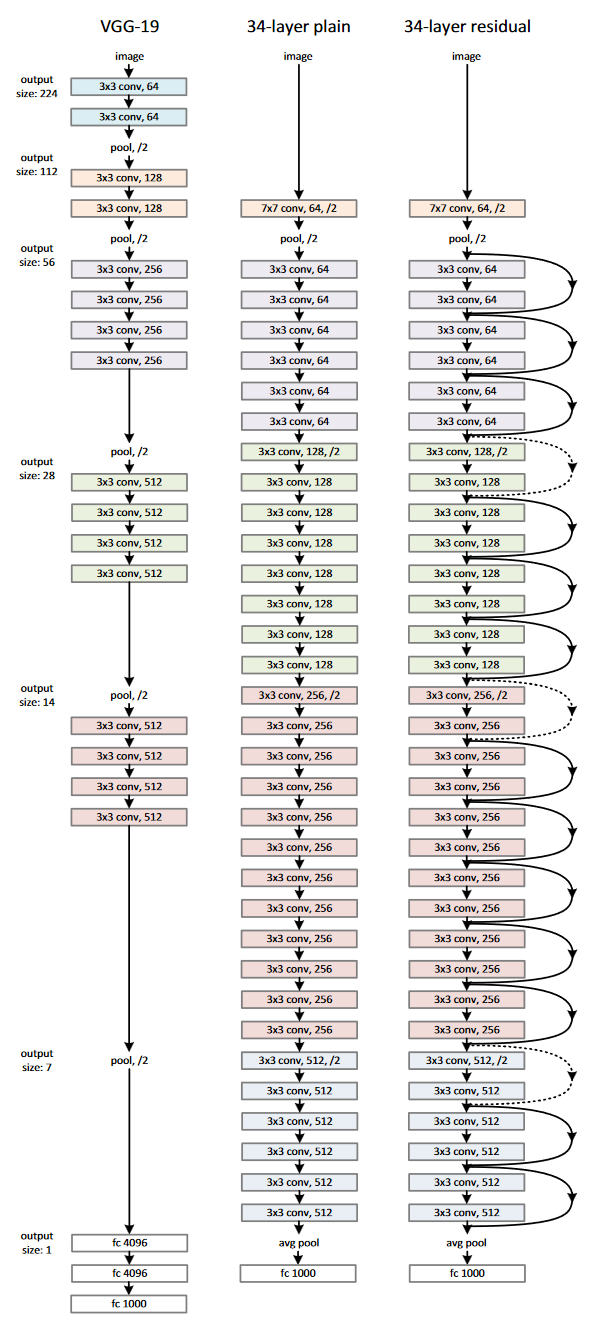
\includegraphics{resnet}
    \caption[Comparison of the architectures of several CNNs.]{\label{fig:resnet}Comparison of the architectures of several CNNs, from left to right: VGG-19, a CNN with 36 layers and a residual CNN with 36 layers. Figure from \cite{he2016deep}.}
\end{marginfigure}


Convolutional networks\index{convolutional network} (CNNs) emerge out of the need to adapt operations to bidimensional data, as well as reduce the computational complexity of dense networks when treating this type of high-dimensional data. Since the matrix used in a dense layer has $n\times m$ parameters, $m$ being the number of variables in the input vector and $n$ the number of variables in the output vector, the amount of floating point operations required to compute the result is $O\left(nm\right)$.

In a CNN, a certain number of matrices typically named \textit{channels} is computed out of the input matrix. Each one is composed of values calculated by convoluting the original matrix with a weight matrix, called \textit{kernel}, which is usually of a fixed small size: $3\times 3$ up to $9\times 9$. Each pixel $(i, j)$ in a filter resulting from convoluting a kernel $K$ over the input $I$ can be computed as follows:
\begin{equation}
    f(i,j)=\left(K\ast I\right)(i,j)=\sum_{m}\sum_{n}I(i-m,j-n)K(m,n)~.
\end{equation}
By keeping $k$, the size of the kernels, notably smaller than the input image, the complexity of convolution is $O(kn)$ and it requires much fewer parameters than matrix multiplication.  This makes CNNs appropriate for image-related tasks such as image classification, segmentation and object detection. They can also extend to tridimensional data such as video segments.


Most current neural network libraries implement cross correlation instead of the discrete convolution, which does not affect the results since equivalent kernels can be learned for it. The operation is still called convolution in most cases, and the only change is a sign flip for $m$ and $n$:
\begin{equation}
    f(i,j)=\left(I\ast K\right)(i,j)=\sum_{m}\sum_{n}I(i+m,j+n)K(m,n)~.
\end{equation}

Convolution is not the only stage performed by CNN. The other important step is \textit{pooling}\index{pooling}. This function outputs a smaller version of its input by summarizing nearby values. For example, max pooling \sidecite{zhou1988computation} takes the maximum out of a rectangle of the input matrix and outputs that as a single value, reducing in this way the size of the matrix.

Computer vision has been one of the fundamental applications of deep learning and CNNs have evolved greatly as a result, with many improvements and extensions such as residual connections (see Figure~\ref{fig:resnet}), breakdown of convolutions into smaller ones \sidecite{7780677}, and pruning strategies \sidecite{lin2019towards}.


\subsubsection{Recurrent networks}

{In a recurrent neural network (RNN)\index{recurrent network}, some parts of the computation of the network at each step, e.g. the output, are fed as input in the next one. This creates a ``memory'' which allows the RNN to remember previous outputs when making predictions. RNNs are used for tasks such as speech recognition and language translation, where the order of the input is important and past outputs are relevant for the next predictions.}

\begin{marginfigure}
    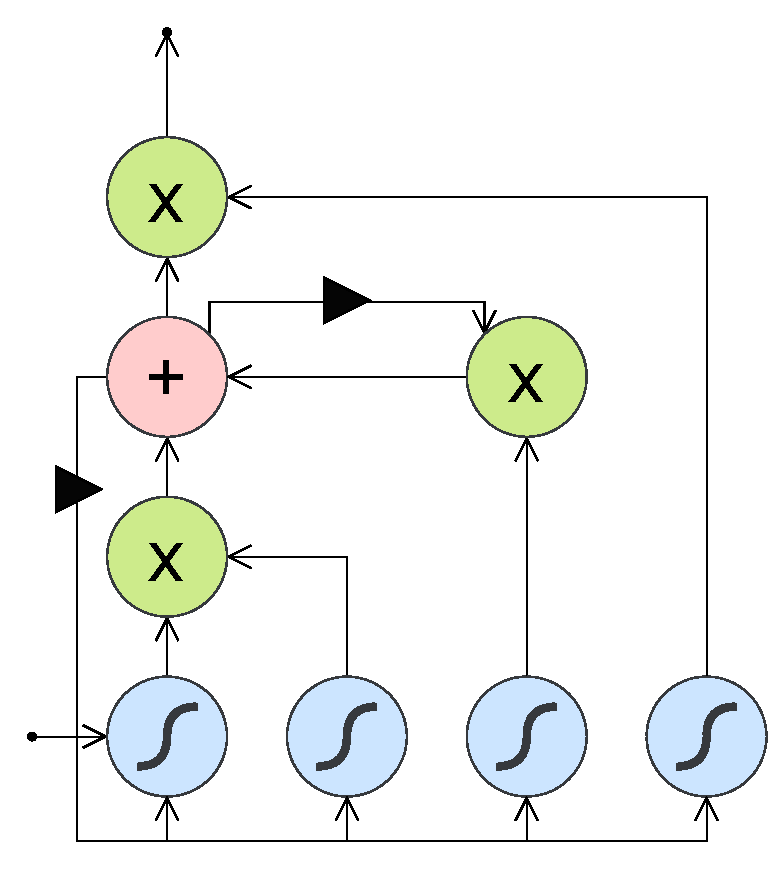
\includegraphics[width=\linewidth]{lstm}
    \caption[Diagram for an LSTM.]{\label{fig:lstm}Diagram for an LSTM where blue units are gates (sigmoidal or tanh activations), green units are products and pink units are sums. Triangles over data flows indicate values that are fed at the next step.}
\end{marginfigure}

A popular kind of RNN units are long short-term memory\index{long short-term memory} (LSTM) units \sidecite{hochreiter1997long}, which add a self-loop controlled (\textit{gated}) by another unit so that the memorized information can be eventually forgotten. See Figure~\ref{fig:lstm} for a detailed schematic of this type of unit.


\subsubsection{Attention and transformers}

Attention\index{attention} mechanisms started in encoder-decoder recurrent networks as a system to identify parts of speech that are more relevant than others within the input data while decoding is in process \sidecite{bahdanau2014neural,luong2015effective}. Instead of compacting all the inputs into an encoded vector and decoding from there, attention allows to have all information available and focus on just the important pieces at each decoding step. There exist several ways of applying attention according to the elements that interact with one another, including self-attention, local attention and global attention.

\begin{marginfigure}
    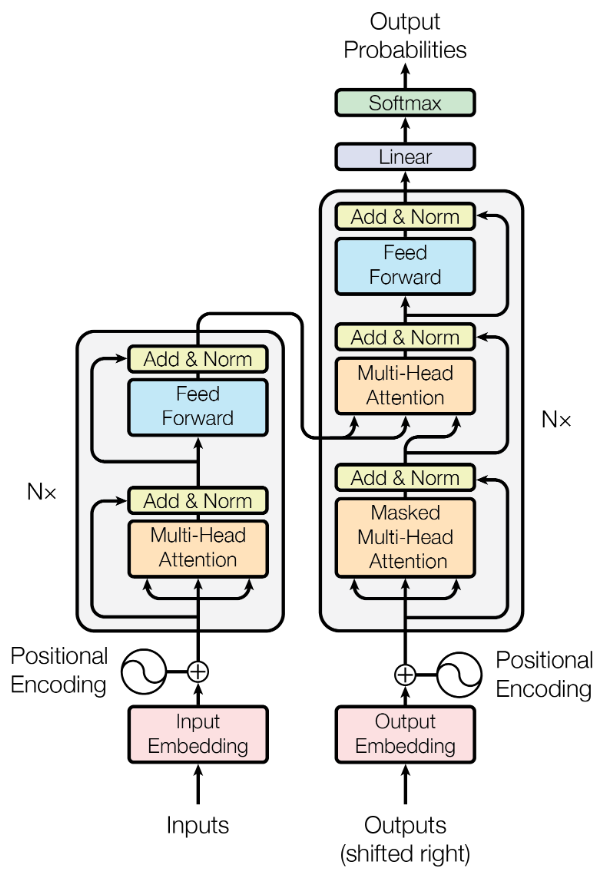
\includegraphics{transformer}
    \caption[Original architecture diagram of the Transformer.]{\label{fig:transformer}Original architecture diagram of the Transformer. Source: \cite{vaswani2017attention}.}
\end{marginfigure}

Based on the concept of attention, transformers\index{transformer} \sidecite{vaswani2017attention} were conceptualized by simply avoiding recurrent units and building the whole network around stacked self-attention operations. Figure~\ref{fig:transformer} shows how a transformer is organized. 
Transformers have been applied beyond machine translation to many other natural language tasks, where they are currently the state of the art \sidecite{devlin-etal-2019-bert}. Some proposals have tackled computer vision as well \sidecite{liu2021swin}, but are being matched in performance by attention-free models such as \sidecite{chen2021cyclemlp}.

\subsection{Network architectures}

Neural layers can be organized in different formations and connected in various ways in order to achieve specific solutions. The structure and connections of a network are known as its architecture\index{architecture}.

\subsubsection{Classifiers and regressors}

Classifiers and regressors are very common types of neural network architectures. The key to obtaining a label output from a network is to stack layers which transform and progressively reduce the dimension of the original data, up to the last layer where the class is selected or a numerical value is predicted. 

Some classification networks are trained and tested against well known benchmarks, becoming a reference for further works and even a basis for other tasks, leveraging the already extracted knowledge by means of \textit{transfer learning}\index{transfer learning}. For instance, the VGG-19 and ResNet networks shown in Figure~\ref{fig:resnet} are standard tools for general image classification.

\subsubsection{Encoder-decoder structures}

There exists a category of deep architectures composed of two components, an \textit{encoder}\index{encoder} and a \textit{decoder}\index{decoder}, where there is an interest in the model operating first with the features in order to obtain higher-level features (encoding) and then developing these features back onto more detailed and specific versions.

For example, when the objective task is to segment the pixels in an image, that is, label each pixel with one of several classes, a possible solution is to compute abstract, high-level features for the image, and use those to classify each pixel next \sidecite{minaee2021image}. This allows to analyze the neighborhoods of each pixel before assigning it to a class, which will probably lead to more cohesive segmentations. Using an encoder-decoder structure, the encoder would compute these low-resolution but high-level features, and the decoder would perform the detailed labeling task out of the extracted information.

Similarly, an encoder-decoder scheme made out of recurrent units, also known as a \textit{sequence-to-sequence} model \sidecite{prabhavalkar2017comparison}, could serve as basis for a language translation system. The encoder would extract an intermediate representation for the meaning of the original sentence and the decoder would transform that onto the target language.

A special subset of encoder-decoder architectures are autoencoders, which are further described next.

\subsubsection{Autoencoders}

\begin{marginfigure}
    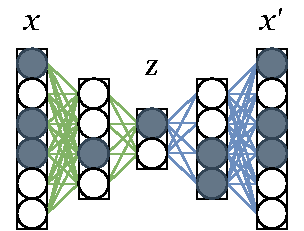
\includegraphics{basic-fc-ae}
    \caption{\label{fig:basicae}Schematic structure of a fully connected autoencoder.}
\end{marginfigure}

Essentially, an \textit{autoencoder}\index{autoencoder} is an encoder-decoder architecture which is trained to map its inputs onto its outputs. Being $f$ the encoder network and $g$ the decoder one, the main objective of an autoencoder would be to match the input data as closely as possible (see Figure~\ref{fig:basicae}):

\begin{equation}
    x\approx g(f(x))
\end{equation}

As a feature learner, the autoencoder trains to extract appropriate features from data by considering that quality features should allow to reconstruct the original data from the encoded vectors.

Different variations can be introduced into the training process and the autoencoder structure in order to extend its functionality. For example, the encoded features can be manipulated to be more sparse, i.e. most of them are equal to 0 for each input vector; the extracted reconstruction can discard noise from the inputs, or it  can model the data as a continuous probability distribution. Article~\ref{ch:paper1} goes into detail about these variants and compares autoencoders to other feature learning methods.

Autoencoders are not limited to the existing variants. Since they are usually based on a penalty function added to the objective that they train to optimize, an expert can define a different penalty function and induce a new behavior on the learned features. This penalty function, unlike the basic objective, can be based on network inputs, outputs, encodings or even external data associated to each instance. This idea is further explored in Article~\ref{ch:paper6}, where three novel autoencoder models are proposed.

Unlike some types of neural networks which are used more commonly such as CNN classifiers or natural language models, autoencoders are not straightforward to implement in current deep learning libraries. This is due to autoencoders having two main output points where most neural networks have one: autoencoders can both encode a feature vector through their middle layer and reconstruct it through their last layer. In spite of this, there are few software tools which act as an abstraction layer over deep learning platforms, giving easier access to autoencoder functionalities. This, along with our developed software package Ruta, is further discussed in Article~\ref{ch:paper2}.

Autoencoders, just like other kinds of networks, can adapt to process data with different structures. As long as the input and output \textit{shapes} of the network coincide, an autoencoder will be able to transform the variables and produce an output as close as possible to the sampled data. In consequence, autoencoders can be made out of dense layers, convolutional layers and recurrent units as detailed in Section~\ref{sec:design}. Other possible structures for problems which could be captured by an adequately built autoencoders are analyzed in Article~\ref{ch:paper3}.

Finally, the utility of autoencoders as feature learners is not limited to helping classification methods by projecting instances to a more useful feature space. As mentioned before, autoencoders may learn noise-resilient representations which allow to restore noisy signals. The reconstruction fidelity can also be used as a sign of anomalous data. Meanwhile, the encoded features can also be binarized to serve as bucket identifiers or treated as a probability distribution to sample new points. All of these applications are explained and demonstrated in Article~\ref{ch:paper5}.

% % \makepart{Published articles}

% % \makearticle{A tutorial on autoencoders}{INFFUS18-AutoencoderTutorial}

% % This paper tackles the variety...

% % \includepdf{INFFUS18-AutoencoderTutorial}

% \pagelayout{margin}
\appendix % From here onwards, chapters are numbered with letters, as is the appendix convention

\makepart{Appendix}

\chapter{Some more blindtext}

\blindtext

%----------------------------------------------------------------------------------------

\backmatter % Denotes the end of the main document content
\setchapterstyle{plain} % Output plain chapters from this point onwards

%----------------------------------------------------------------------------------------
%	BIBLIOGRAPHY
%----------------------------------------------------------------------------------------

% The bibliography needs to be compiled with biber using your LaTeX editor, or on the command line with 'biber main' from the template directory

\defbibnote{bibnote}{Here are the references in citation order.\par\bigskip} % Prepend this text to the bibliography
\printbibliography[heading=bibintoc, title=Bibliography, prenote=bibnote] % Add the bibliography heading to the ToC, set the title of the bibliography and output the bibliography note

%----------------------------------------------------------------------------------------
%	INDEX
%----------------------------------------------------------------------------------------

% The index needs to be compiled on the command line with 'makeindex main' from the template directory

\printnomenclature % Output the index

\end{document}
